\pagenumbering{roman}
%%%%%%%%%%%%%%%%%%%%%%%%%%%
% Diplomaterv-kiiras (ezt adjak, bele kell kötni a diplomába)
%%%%%%%%%%%%%%%%%%%%%%%%%%%
\begin{center}

\textbf{BUDAPEST UNIVERSITY OF TECHNOLOGY AND ECONOMICS}

\medskip


\includegraphics[width=8.79cm]{images/bme.pdf}

\medskip

\textbf{FACULTY OF ELECTRICAL ENGINEERING AND INFORMATICS\\SOFTWARE ENGINEERING}

 \vspace{2cm}
 \Large\textbf{\cim}

 \vspace{6mm}
 \textbf{\nev} \\
 \texttt{<vsza@vsza.hu>} \\ \strut \\

 \Large\textbf{THESIS STUDY}

\end{center}

\vfill

Consultant:

\begin{center}
\konzulens\\ \konzbeoszt

\vspace{96pt}

December 2011
\end{center}

% \vspace{6mm}
% \begin{tabular}{p{80mm}l}
% A záróvizsga tárgyai:   & Első tárgy \\
%                         & Második tárgy \\
%                         & Harmadik tárgy
%  \end{tabular}
%
%  \vspace{6mm}
%  \begin{tabular}{p{80mm}l}
%  A tervfeladat kiadásának napja:         &  \\
%  A tervfeladat beadásának határideje:    &
%  \end{tabular}
%
% \vfill
%
% \begin{center}
% \begin{tabular}{cc}
%  \makebox[7cm]{\emph{dr.\ Görgényi András}}    & \makebox[7cm]{\emph{dr.\ Péceli Gábor}} \\
%  \makebox[7cm]{adjunktus, diplomaterv felelős} & \makebox[7cm]{egyetemi tanár, tanszékvezető}
% \end{tabular}
% \end{center}
%
%  \vspace{6mm}
%  \begin{tabular}{p{80mm}l}
%  A tervet bevette:           & \\
%  A terv beadásának dátuma:   & \\
%  A terv bírálója:            &
%  \end{tabular}


 \thispagestyle{empty}
 \blankpage

\selectlanguage{magyar}
%%%%%%%%%%%%%%%%%%%%%%%%%%%
% Diplomaterv-kiiras melleklete (ezt is adjak, bele kell kötni a diplomába)
%%%%%%%%%%%%%%%%%%%%%%%%%%%
 \begin{textblock*}{\paperwidth}(0mm,0mm)
    \noindent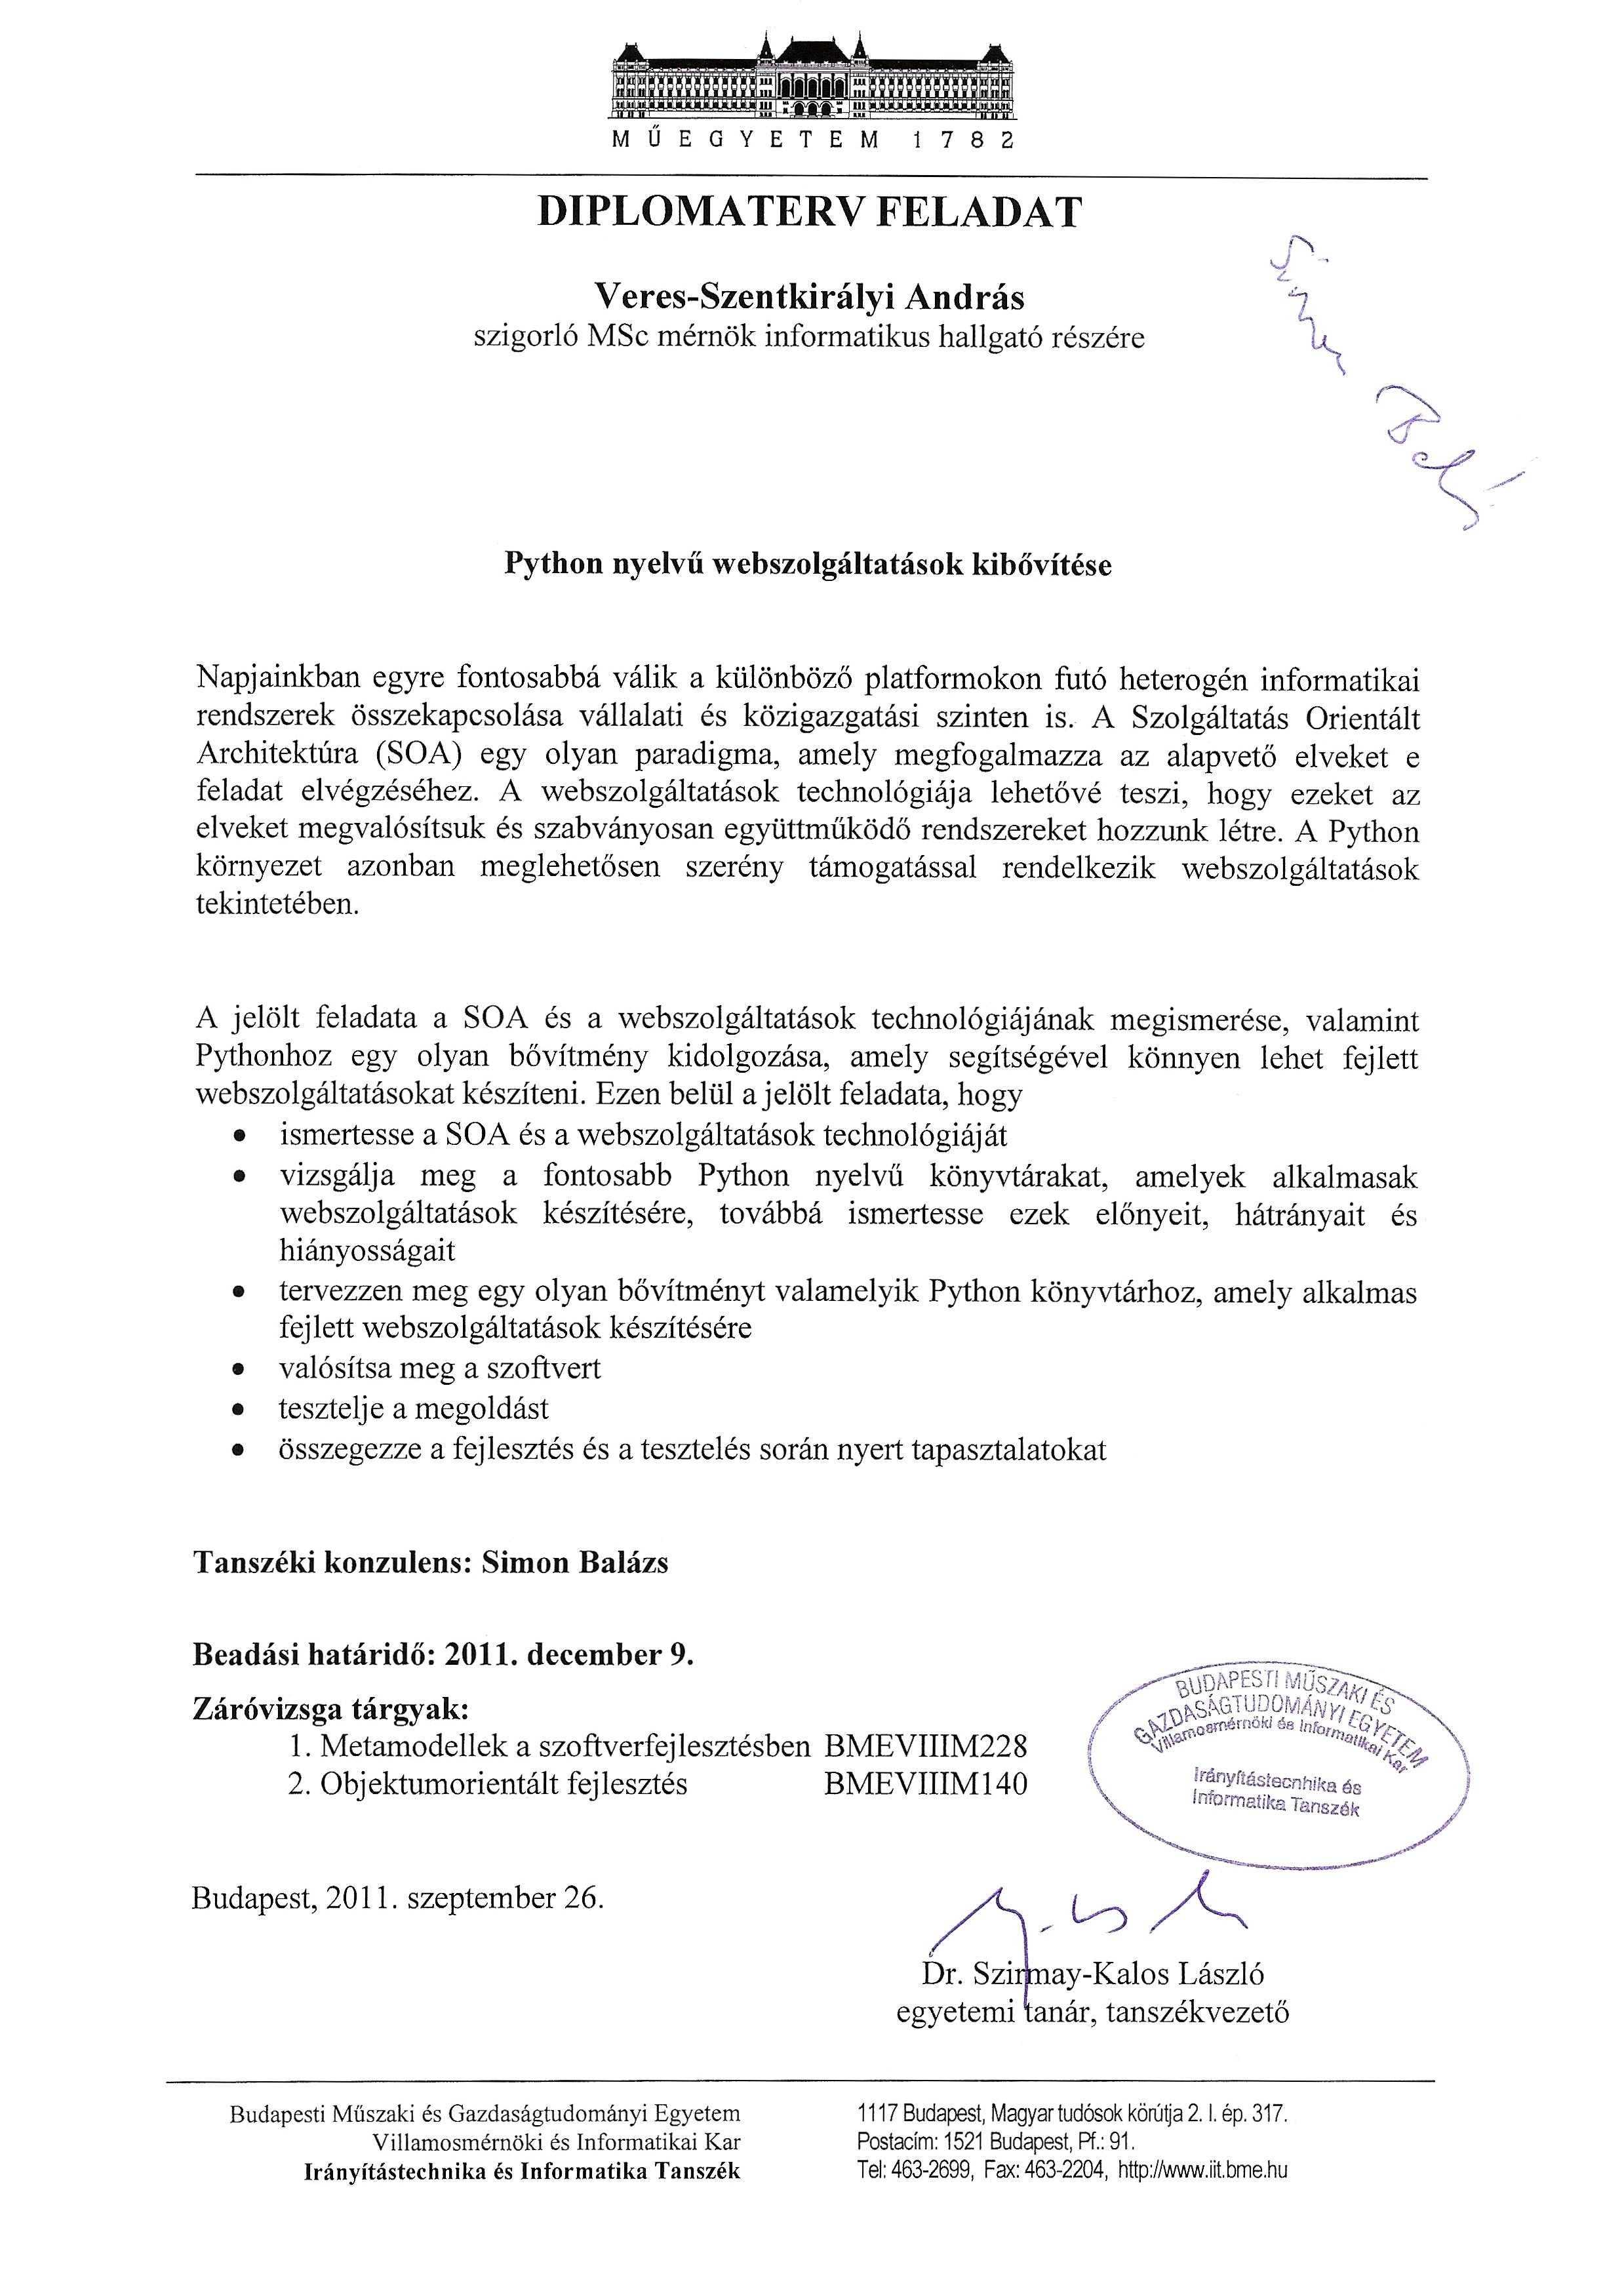
\includegraphics[width=\paperwidth,height=\paperheight]{images/feladat-retouched.jpg}
	\end{textblock*}
	\mbox{}
 \blankpage

%%%%%%%%%%%%%%%%%%%%%%%%%%%
% Nyilatkozat
%%%%%%%%%%%%%%%%%%%%%%%%%%%
\def\abstractname{Nyilatkozat}
\begin{abstract}

\noindent
Alulírott \emph{Veres-Szentkirályi András}, szigorló hallgató kijelentem,
hogy ezt a diplomatervet meg nem engedett segítség nélkül, saját  magam
készítettem, csak a megadott forrásokat (szakirodalom, eszközök, stb.)
használtam fel. Minden olyan  részt, amelyet szó szerint, vagy azonos
értelemben, de átfogalmazva más forrásból átvettem, egyértelműen, a
forrás megadásával megjelöltem.

Hozzájárulok, hogy a jelen munkám alapadatait (szerző(k), cím, angol és magyar
nyelvű tartalmi kivonat, készítés éve, konzulens(ek) neve) a BME VIK nyilvánosan
hozzáférhető elektronikus formában, a munka teljes szövegét pedig az egyetem
belső hálózatán keresztül (vagy autentikált felhasználók számára) közzétegye.
Kijelentem, hogy a benyújtott munka és annak elektronikus verziója megegyezik.
Dékáni engedéllyel titkosított diplomatervek esetén a dolgozat szövege csak 3 év
eltelte után válik hozzáférhetővé.
\begin{flushright}
 \vspace*{1cm}
 \makebox[7cm]{\rule{6cm}{.4pt}}\\
 \makebox[7cm]{\emph{Veres-Szentkirályi András}}\\
 \makebox[7cm]{hallgató}
\end{flushright}
\end{abstract}

%%%%%%%%%%%%%%%%%%%%%%%%%%%
% Tartalomjegyzek
%%%%%%%%%%%%%%%%%%%%%%%%%%%
\selectlanguage{english}
\tableofcontents

%%%%%%%%%%%%%%%%%%%%%%%%%%%
% Kivonat
%%%%%%%%%%%%%%%%%%%%%%%%%%%
\def\abstractname{Kivonat}
\selectlanguage{magyar}
\begin{abstract}
\addcontentsline{toc}{chapter}{Kivonat}
``Én távolabbra láthattam, de csak azért, mert óriások vállán álltam'' -- Isaac Newton több mint 300 éves üzenete jól illeszthető a szolgáltatások együttműködésének kialakítása mögött rejlő motivációval. Ahogy egyre fejlettebb szolgáltatások kerültek a piacra, a versenyelőny megtartásának egy jó módja ezek összekapcsolása, ezáltal újszerű, összetett termékek létrehozása. A technológia folyamatos fejlődése egyszerre teremtett sok-sok eltérő platformot és az ezek közti hatékony együttműködést lehetővé tévő szabványokat, mint a DCOM, a CORBA és az XML-RPC.

A bábeli zűrzavarra megoldás a webszolgáltatások technológiája, mely a SOAP-ot használja az üzleti üzenetek szabványos kódolására, és a világháló kapcsán már bevált, egyszerű és kiforrott szállítási mechanizmusok segítségével juttatja el azokat a címzetthez. Bár az Internet nyíltsága végtelen lehetőségeket rejt, megvannak a veszélyei is, így további szabványok jelentek meg, többek között az üzenetek hitelességének biztosítására.

Bár a nyílt szabványok, mint a SOAP, WSDL és társai egy platform-független megoldást alapozhattak volna meg, ezek fejlesztői környezetek körében élvezett támogatása közel sem egyenletes. Például a Python, egy valódi közösségi projekt, a szükséges minimumnál alig nyújt több támogatást fejlett SOAP webszolgáltatások készítéséhez, így az ezt igénylő projektek körében kevésbé népszerű választás, egyéb pozitív tulajdonságai ellenére.

Diplomatervemben bemutatom a Szolgáltatás Orientált Architektúra történetét és elveit, majd részletezésre kerülnek a webszolgáltatások, azon belül is a fejlettek. A Python környezetről is lehull a lepel, többek között áttekintem a jelenleg rendelkezésre álló, SOA megoldások készítésére alkalmas könyvtárakat mind szolgáltatási, mind fogyasztói oldalról. A felsorolást egy összegzés zárja, mellyel célom rávilágítani a fejlesztések szükségességére.

Az általam továbbfejlesztésre kiválasztott könyvtár, a SUDS bemutatása során mind a magas szintű fejlesztői interfész, mind a belső működés áttekintésre kerül, rámutatva a bővítés kiindulópontjaként használható csonka részekre. A bővítményre vonatkozó terveim és azok megvalósításának bemutatását követően szó esik a tesztkörnyezetről is, melynek elkészítésével az volt a célom, hogy bebizonyosodjon, a fejlesztés eredménye teljesíti a legfontosabb követelményt: az interoperabilitást. Végül a megoldás színvonala a felhasznált idő és hálózati forgalom mértéke alapján került értékelésre, a diplomatervet pedig tapasztalataim összegzése és továbbfejlesztési lehetőségek zárják.
\end{abstract}


%%%%%%%%%%%%%%%%%%%%%%%%%%%
% Abstract
%%%%%%%%%%%%%%%%%%%%%%%%%%%
\selectlanguage{english}
\begin{abstract}
\addcontentsline{toc}{chapter}{Abstract}
``If I have seen further it is only by standing on the shoulders of giants'' -- Isaac Newton's more than 300-year-old message is a great parallel with the motivation behind service interoperation. As more advanced services were developed, one way of improving them was to interconnect them to combine their powers into more exciting products. Continuous advancement of technology created diverging platforms, and simultaneously provided standards allowing efficient co-operation such as DCOM, CORBA and XML-RPC.

One of the solutions for this Babel-like chaos were web services using SOAP to encode business messages in a standardized way and to reuse simple and mature transport mechanisms proven useful by the World Wide Web to carry them between the recipients. While the openness of Internet offers vast opportunities, it also has its dangers, which caused additional standards to be developed, among others, for message authenticity.

Although the open standards of SOAP, WSDL and others could have been the foundation of a platform-independent solution, not every environment used for software development supports it equally. Python, a truly community-driven project is one of them, providing little more than minimal support for advanced SOAP web services, making it a less favored selection for projects needing this capability, despite its unique treats.

In this thesis, the history and principles of Service-Oriented Architecture are presented, then the scope is focused on web services, and further on to advanced ones. Then the Python environment is introduced, including the current libraries for implementing SOA solutions both on the service and consumer side. This part ends with a quick summary that makes the reasons for improvements clear.

My selection for improvement, SUDS is presented next, looking at both its high-level view and its internals, showing the possible stubs awaiting improvement. The plans and implementation details of my enhancements are introduced right after, including a testbed to make sure the new features fulfill the most important requirement: interoperation. In the end, the whole solution is evaluated using measurements of both timing and network traffic, concluding the thesis with my observations and ideas for future improvement.
\end{abstract}
